% Figure from MATH 591 notes, section 68 (the flow domain of the escape example). Added, not from lecture (Lecture 23 delivery).
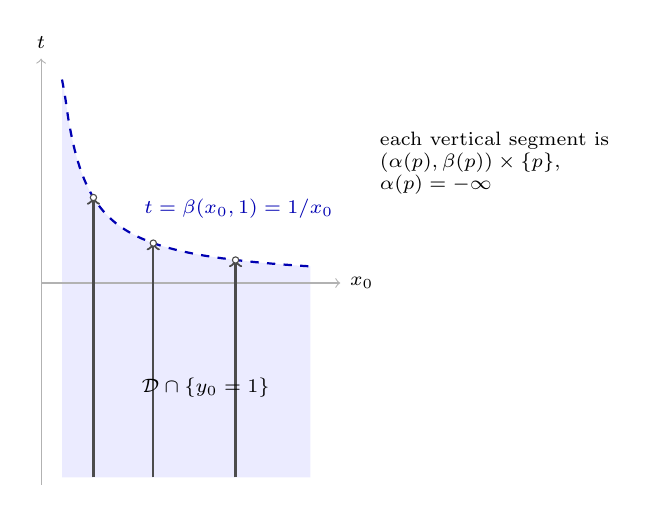
\begin{tikzpicture}[scale=0.95]
\fill[blue!8] (0.28,-2.6) -- plot[smooth] coordinates {(0.280,2.720) (0.322,2.484) (0.364,2.197) (0.406,1.970) (0.448,1.785) (0.490,1.632) (0.532,1.503) (0.574,1.393) (0.616,1.298) (0.658,1.215) (0.700,1.142) (0.742,1.078) (0.784,1.020) (0.826,0.968) (0.868,0.921) (0.910,0.879) (0.952,0.840) (0.994,0.804) (1.036,0.772) (1.078,0.742) (1.121,0.714) (1.163,0.688) (1.205,0.664) (1.247,0.642) (1.289,0.621) (1.331,0.601) (1.373,0.583) (1.415,0.565) (1.457,0.549) (1.499,0.534) (1.541,0.519) (1.583,0.505) (1.625,0.492) (1.667,0.480) (1.709,0.468) (1.751,0.457) (1.793,0.446) (1.835,0.436) (1.877,0.426) (1.919,0.417) (1.961,0.408) (2.003,0.399) (2.045,0.391) (2.087,0.383) (2.129,0.376) (2.171,0.368) (2.213,0.361) (2.255,0.355) (2.297,0.348) (2.339,0.342) (2.381,0.336) (2.423,0.330) (2.465,0.325) (2.507,0.319) (2.549,0.314) (2.591,0.309) (2.633,0.304) (2.675,0.299) (2.717,0.294) (2.759,0.290) (2.802,0.286) (2.844,0.281) (2.886,0.277) (2.928,0.273) (2.970,0.269) (3.012,0.266) (3.054,0.262) (3.096,0.258) (3.138,0.255) (3.180,0.252) (3.222,0.248) (3.264,0.245) (3.306,0.242) (3.348,0.239) (3.390,0.236) (3.432,0.233) (3.474,0.230) (3.516,0.228) (3.558,0.225) (3.600,0.222)} -- (3.6,-2.6) -- cycle;
\draw[->, gray!60] (0,0) -- (4.0,0) node[right, font=\scriptsize, text=black] {$x_0$};
\draw[->, gray!60] (0,-2.7) -- (0,3.0) node[above, font=\scriptsize, text=black] {$t$};
\draw[blue!70!black, thick, dashed] plot[smooth] coordinates {(0.280,2.720) (0.322,2.484) (0.364,2.197) (0.406,1.970) (0.448,1.785) (0.490,1.632) (0.532,1.503) (0.574,1.393) (0.616,1.298) (0.658,1.215) (0.700,1.142) (0.742,1.078) (0.784,1.020) (0.826,0.968) (0.868,0.921) (0.910,0.879) (0.952,0.840) (0.994,0.804) (1.036,0.772) (1.078,0.742) (1.121,0.714) (1.163,0.688) (1.205,0.664) (1.247,0.642) (1.289,0.621) (1.331,0.601) (1.373,0.583) (1.415,0.565) (1.457,0.549) (1.499,0.534) (1.541,0.519) (1.583,0.505) (1.625,0.492) (1.667,0.480) (1.709,0.468) (1.751,0.457) (1.793,0.446) (1.835,0.436) (1.877,0.426) (1.919,0.417) (1.961,0.408) (2.003,0.399) (2.045,0.391) (2.087,0.383) (2.129,0.376) (2.171,0.368) (2.213,0.361) (2.255,0.355) (2.297,0.348) (2.339,0.342) (2.381,0.336) (2.423,0.330) (2.465,0.325) (2.507,0.319) (2.549,0.314) (2.591,0.309) (2.633,0.304) (2.675,0.299) (2.717,0.294) (2.759,0.290) (2.802,0.286) (2.844,0.281) (2.886,0.277) (2.928,0.273) (2.970,0.269) (3.012,0.266) (3.054,0.262) (3.096,0.258) (3.138,0.255) (3.180,0.252) (3.222,0.248) (3.264,0.245) (3.306,0.242) (3.348,0.239) (3.390,0.236) (3.432,0.233) (3.474,0.230) (3.516,0.228) (3.558,0.225) (3.600,0.222)};
\node[blue!70!black, font=\scriptsize, anchor=west] at (1.25,0.99) {$t = \beta(x_0, 1) = 1/x_0$};
\foreach \x in {0.7,1.5,2.6} { \draw[thick, black!70, ->] (\x,-2.6) -- (\x,{0.8/\x}); \fill[white, draw=black!70] (\x,{0.8/\x}) circle (1.2pt); }
\node[font=\scriptsize, align=center] at (2.2,-1.4) {$\mathcal{D} \cap \{y_0 = 1\}$};
\node[font=\scriptsize, anchor=west, align=left] at (4.4,1.6) {each vertical segment is\\ $(\alpha(p), \beta(p)) \times \{p\}$,\\ $\alpha(p) = -\infty$};
\end{tikzpicture}
